\chapter{Introduction to the split-operator method for vortex simulations}
\label{ch:splitop}

The split-operator method is a pseudo-spectral technique for solving partial differential equations and is particularly useful for several nonlinear partial differential equations such as the Gross--Pitaevskii Equation (GPE),

$$
i \hbar \frac{\partial \Psi(\mathbf{r},t)}{\partial t} = \left(\frac{p^2}{2m} + V_0 + g |\Psi(\mathbf{r},t)|^2 \right)\Psi(\mathbf{r},t)
$$

where $\mathbf{r}$ is a position vector, $\Psi(\mathbf{r},t)$ is a many-body quantum wavefunction, $p = -i\hbar\nabla$ is the momentum operator, $V_0$ is the trapping potential, g = $\frac{4\pi\hbar^2 a_s}{m}$, $a_s$ is the scattering length of the atomic species, and $m$ is the mass.

By solving the GPE with time, we can determine the dynamics of Bose--Einstein Condensates (BECs).
The states found with the GPE are virtually identical to those found in experiments.

One important technique for solving the GPE is the pseudospectral split-operator method, which requires splitting the hamiltonian into separate operators in position and momentum space and operating on the wavefunction in the appropriate space.
To understand how this is done, it is important to first discuss the mathematical formalism used to transform between position and momentum space: the Fourier Transform.

\section{The Schr\"odinger equation and the Hamiltonian}
Quantum particles are often described by their wavefunction, $\Psi(\mathbf{r},t)$, where $\mathbf{r}$ is a position-space variable and $t$ is time.
This does not have a simple physical interpretation; however, the wavefunction density, $|\Psi(\mathbf{r},t)|^2$, can be interpreted as a probability distribution in position-space, where peaks represent areas where quantum particles are likely to be found.
As with most probability distributions,

\begin{equation}
    \label{eqn:norm}
    \int_\infty^\infty |\Psi(\mathbf{r},r)|^2 d\mathbf{r} = N,
\end{equation}

\noindent where $N$ is the number of particles in the system.
For certain simulations with the SSFM method, it is important to ensure the quantum system is normalized correctly and Equation~(\ref{eqn:norm}) is used for this purpose.
This will be discussed in further detail in Chapter~\ref{ch:splitop}.

For the purposes of this body of work, we can simulate the dynamics of a quantum system by solving the Schr\"odinger equation,

\begin{equation}
    i\hbar\frac{\partial\Psi(\mathbf{r},t)}{\partial t} = \left(\frac{p^2}{2m} + V_0\right) \Psi(\mathbf{r},t)
    \label{eqn:schrody}
\end{equation}

\noindent where $m$ is the mass of the atomic system, $p = -i\hbar\nabla$ is the momentum operator, and $V_0$ is the trapping potential.
This is a partial differential equation that relates the change in the wavefunction with time on the left-hand side to physical arguments like momentum and position on the right.
For this reason, the operators on the right-hand side are often described as the \textit{Hamiltonian operator}, 

\begin{equation}
\mathcal{\hat H} = \frac{p^2}{2m} + V_0
\end{equation}

\noindent which noticeably has two separate operators: one in momentum-space ($\mathcal{\hat H}_p = \frac{p^2}{2m}$) and another in position-space ($\mathcal{\hat H}_v = V_0$).
The Hamiltonian describes how the quantum system evolves with time, and in this work, we modify the Hamiltonian to match the various quantum systems we would like to simulate.

\begin{figure}

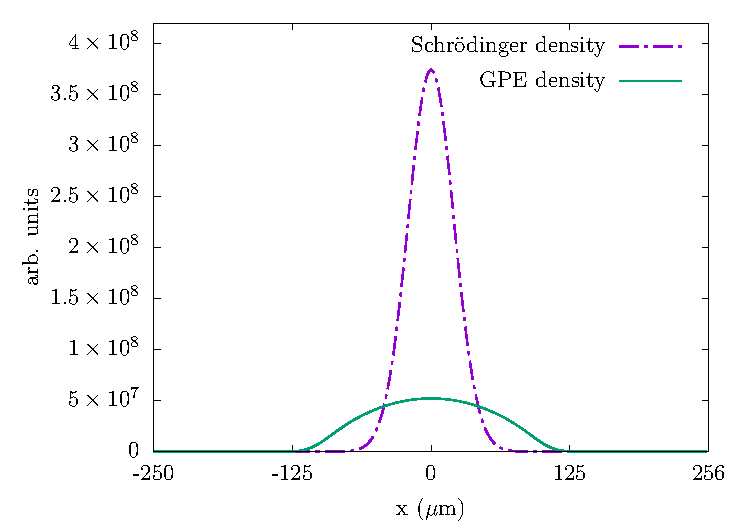
\includegraphics[width = \textwidth]{data/qs/SHO/SHO.pdf}

\caption{Simulated results from ground-state evolution from the split-step Fourier method after 10,000 steps. Here, we use a Rubidium 87 atom with $\omega_x = 1$Hz on a 256-point grid of size 200 $\mu$m. The wavefunction has been normalized such that $\int_{-\infty}^\infty|\Psi|^2 dx = 1$, which provides arbitrary units. We have scaled the potential by $m \omega_x^2 dx^2$ to match these units. This simulation was performed with the GPUE codebase \cite{schloss2018}.}
\label{fig:SHO}
\end{figure}

When the quantum system is in its lowest energy state, the probability distribution will often follow the trapping potential.
For example, in the case of the simple harmonic oscillator in one dimension, $V_0 = m \omega_x x^2$, where $\omega_x$ is the trapping frequency in the $x$-dimension and describes the tightness of the trap.
Figure~\ref{fig:SHO} shows the lowest energy state, also called the \textit{ground state} of a quantum system consisting of a single particle.
Notably, the quantum particle rests in the center of the trap and if the trap is moved, the particle will move with it and oscillate about the new trap location.
Many quantum engineering systems require precise control of the trapping potential to manipulate quantum systems~\cite{menchon2016}, and we will discuss two such methods (quantum optimal control~\cite{werschnik2007} and shortcuts to adiabaticity~\cite{guery2019}) in Chapter~\ref{ch:1d}.

Quantum systems do now always have a straightforward interpretation, and $\Psi(\mathbf{r},t)$ is a complex-valued object with operators in both position and momentum space.
As such, it is important to discuss fundamental relationships between position and momentum space in order to better understand quantum systems, and ultimately how the SSFM acts in both spaces.

\section{The Heisenberg uncertainty principle}

\jrs{NC; Maybe move this to the splitop chapter, as well?}

The Heisenberg uncertainty principle is a relation between the position and momentum components of a quantum system.
This principle simply states that

$$
\sigma_x \sigma_p \geq \frac{\hbar}{2},
$$

where $\sigma_x$ and $\sigma_p$ are the standard deviations of the position-space and momentum-space distributions for a quantum system.
Because these two variables are inversely proportional, this can be interpreted to mean that as the measurement in one domain becomes more precise, the measurement in the conjugate domain becomes less so.
This is historically interesting, as it seems to provide the fundamental limit to the precision by which the momentum or position of a quantum particle can be measured to be Planck's constant $h$.

For the purposes of this work, we do not need to delve too deeply into the interpretation of this principle.
Instead, we need to find an appropriate mathematical formalism that allows for us to easily recreate the same properties, and thus develop a method for transforming between position and momentum space for quantum simulations.
In this case, we can see this relation simply by performing a Fourier transform on a set of gaussians with an increasing standard deviation, as shown in Figure~\ref{fig:uncertain}

\begin{figure}

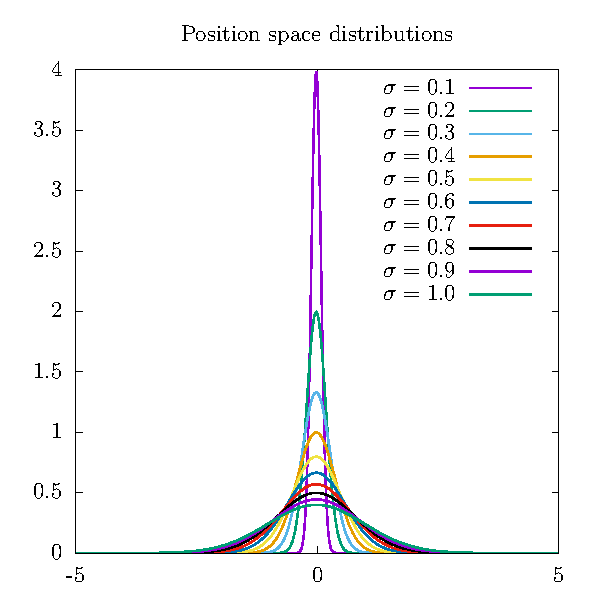
\includegraphics[width = 0.5\textwidth]{data/qs/Heisenberg/position.pdf}
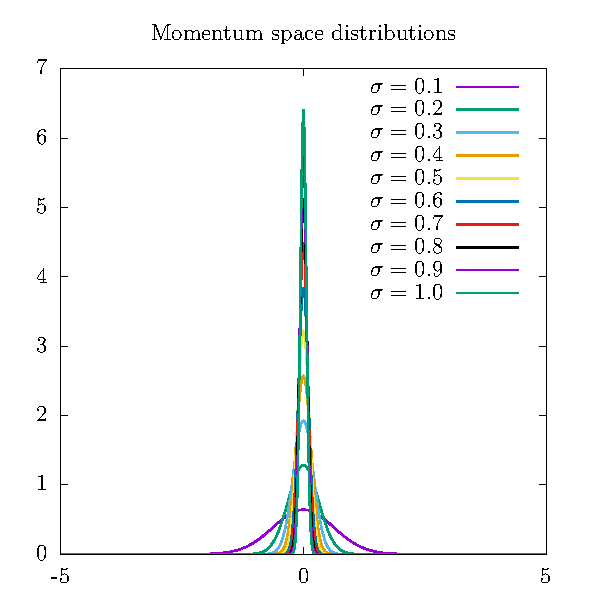
\includegraphics[width = 0.5\textwidth]{data/qs/Heisenberg/momentum.pdf}

\caption{A series of Gaussians with increasing standard deviation. We see that as the standard deviation for the Gaussians in position space increase, the standard devations in momentum space decrease.}
\label{fig:uncertain}
\end{figure}


As such, it is worth exploring the Fourier transform, itself, and discussing its various applications.
Further discussions about numerical methods for implementing the Fourier transform will be discussed in Chapter~\ref{ch:splitop}.


\section{The Fourier transform}

\begin{figure}

\begin{centering}

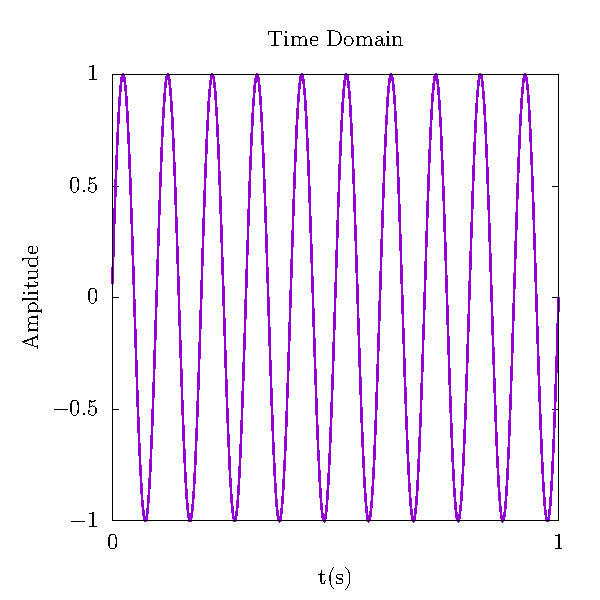
\includegraphics[width = 0.48\textwidth]{data/splitop/fourier/sine_wave.pdf}
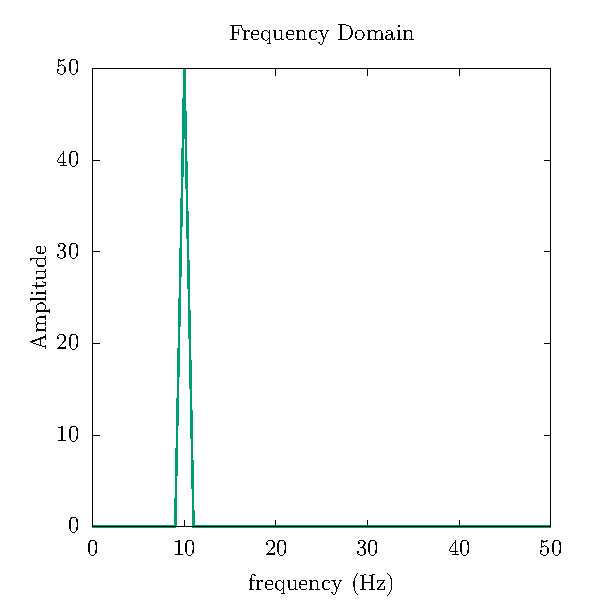
\includegraphics[width = 0.48\textwidth]{data/splitop/fourier/sine_fft.pdf}

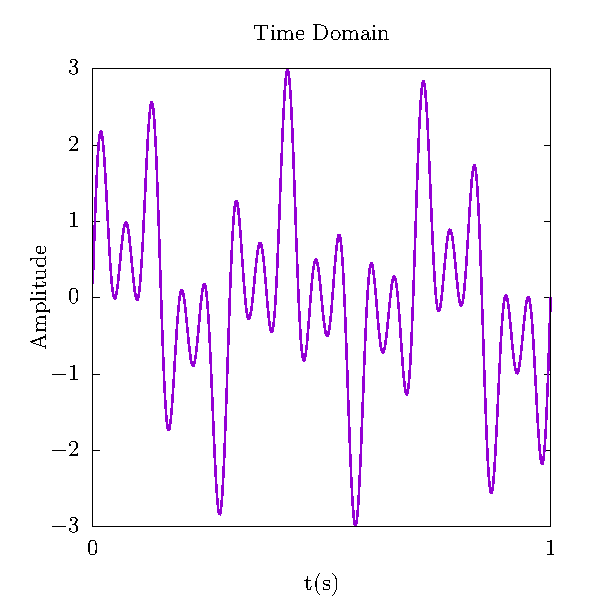
\includegraphics[width = 0.48\textwidth]{data/splitop/fourier/3_waves.pdf}
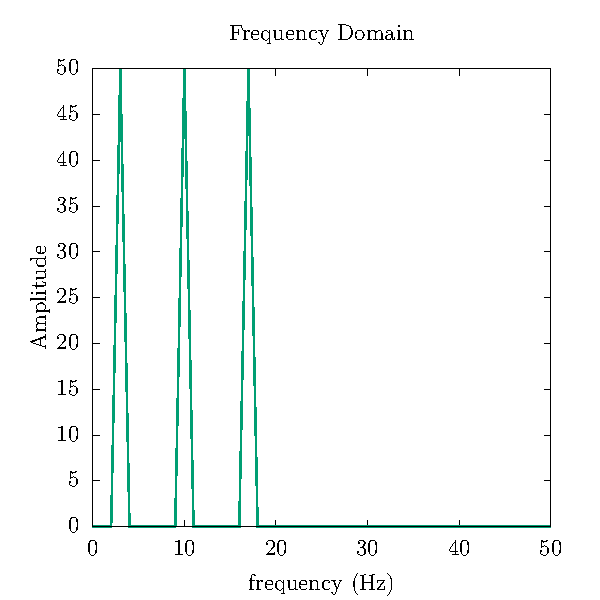
\includegraphics[width = 0.48\textwidth]{data/splitop/fourier/3_fft.pdf}

\end{centering}

\caption{Depiction of a fourier transform, first with a sine wave with a frequency of 10 Hz, and then with a combination of 3 waves of frequencies 3, 10, and 17 Hz. Note that the signal in the Frequency domain is a sparse representation of the singnal in the time domain.}
\label{fig:FT}
\end{figure}

The Fourier transform is a fundamental mathematical technique that lies at the heart of signal processing, and is used for numerous methods, including SSFM, which will be discussed further in Chapter~\ref{ch:splitop}.
Because it is such a fundamental technique, there are many intuitive descriptions for interpreting the Fourier transform, and it would not be worthwhile to discuss all of these explanations here.
In most cases, the Foureir transform is introduced as a transformation between the time domain and frequency domain; however, as we discussed in the previous section, it can also transform between any conjugate parameters, such as position and momentum.
As an example, if we have some wave in the time domain with some frequency $\omega$, such as $\sin(20\pi\omega)$, we can plot the signal fully in the time-domain; however, the signal changes to a single peak in the frequency domain, as shown in Figure~\ref{fig:FT}(a).

In fact, every point in the frequency domain corresponds to another distinct wave in the time-domain.
As such, we can decompose most wave-like signals into a sparse set of delta-like peaks in the frequency domain, and this can be seen in Figure~\ref{fig:FT}(b).
In general, if we have a set of parameters that are ``full'' in one domain, it is likely sparse in it's conjugate domain.
This sparsity has been used for many applications, including compressed sensing, which allows us to reconstruct high-resolution data from low-resolution ouput in a separate domain~\cite{baraniuk2011}.
We will discuss this in more depth in Chapter~\ref{ch:splitop} when we discuss the compressed split-step Fourier method, which applies tecniques in compressive sensing to the SSFM \cite{bayindir2015}.

Mathematically, the Fourier transform can be represented as,

$$
\mathcal{F}(\xi) = \int_{-\infty}^{\infty}f(t)e^{-2\pi i t \xi}dt
$$

\noindent and the inverse Fourier transform can be represented as,

$$
f(t) = \int_{-\infty}^{\infty}\mathcal{F}(\xi)e^{2\pi i t \xi}d\xi
$$

\noindent where $t$ is an element in the time-domain, $\xi$ is an element in the frequency domain, $f(t)$ is a time-domain function, and $\mathcal{F}(\xi)$ is a corresponding frequency-domain function.
In almost all cases related to this work, it is equally important to discuss the Discrete Fourier Transform (DFT), for which the forward transform is,

$$
X_k = \sum_{n=0}^{N-1} x_n e^{-2 \pi i k n / N}
$$

\noindent and the inverse transform is,

$$
x_n = \frac{1}{N} \sum_{k=0}^{N-1} X_k e^{2 \pi i k n / N}
$$

\noindent where $X_k$ and $x_n$ represent the frequency and time domain signals, respectively, $k$ is a component in the frequency domain, $x$ is a component in the time domain, and N is the total number of elements in the signal.
Though the primary difference between these two definitions is that the DFT replaced the integral of the Fourier transform with a sum, the DFT also allows for the computational investigation of signal processing, as it can now be interpreted as a sum and matrix multiplication.
ADD DISCUSSION ON DFT MATRIX? PROBABLY NOT RELEVANT...
Unfortunately, this comes at a huge cost for complexity, as the matrix multiplication, alone, is of the order of $\mathcal{O}(n^3)$, and with the sum, the DFT has a heafty computational complexity of $\mathcal{O}(n^4)$, assuming a square signal.

Luckily, there have been several successful attempts to create a Fast Fourier Transform (FFT), including the Cooley-Tukey method, that was first discovered by Gauss and then later contemporized by Cooley and Tukey when they independently discovered it \cite{cooley1965}.
This method is not straightforwardly parallelizable; however, it has become so fundamental to signal processing, that it has become incredibly well-optimized with several libraries, including FFTW~\cite{frigo1998} and CuFFT~\cite{fatica2008} for distributed and GPU calculations, respectively.

We will discuss the Cooley-Tukey method, itself, along with different parallelization methods for multi-GPU simulations in Chapter~\ref{ch:splitop}.
For now, we will turn our focus to attributes of the physical systems we will be simulating throughout this work, ultracold atoms.


\section{The split-operator method}

As mentioned, the split-operator method splits the Hamiltonian into separate operators and uses the Fourier transform to ensure that these operators work on the wavefunction in the appropriate space.

First, we assume a somewhat general solution to our wavefunction,

$$
\Psi(\mathbf{r},t + dt) = \left[e^{-\frac{i\hat{H}dt}{\hbar}}\right]\Psi(\mathbf{r},t) = \left[e^{-\frac{i(\hat{H}_r + \hat{H}_k)dt}{\hbar}}\right]\Psi(\mathbf{r},t)
$$

and assume we are simulating our system by a series of small timesteps ($dt$), we can perform similar splitting by using the Baker-Campbell-Housdorff formula:

$$
\Psi(\mathbf{r},t+dt) = \left[e^{-\frac{i\hat{H}_rdt}{\hbar}}e^{-\frac{i\hat{H}_kdt}{\hbar}}e^{-\frac{[i\hat{H}_r, i\hat{H}_k]dt^2}{2}}\right]\Psi(\mathbf{r},t)
$$

This accrues a small amount of error ($dt^2$) related to the commutation of the real and momentum-space components of the Hamiltonian, which is a noticeably high.
In order to change the $dt^2$ error to $dt^3$, we can split the system by performing a half-step in position space before doing a full-step in momentum space, through a process called \textit{Strang Splitting} like so:

$$
\Psi(\mathbf{r},t+dt) = \left[e^{-\frac{i\hat{H}_rdt}{2\hbar}}e^{-\frac{i\hat{H}_kdt}{\hbar}}e^{-\frac{i\hat{H}_rdt}{2\hbar}} \right]\Psi(\mathbf{r},t) + \mathcal{O}(dt^3)
$$

We can then address each part of this solution in chunks, first in position space, then in momentum space, then in position space again by using Fourier Transforms.
Which looks something like this:

$$
\Psi(\mathcal{r}, t+dt) = \left[\hat{U}_r\left(\frac{dt}{2}\right)\mathcal{F}^{-1}\left[\hat{U}_k(dt) \mathcal{F} \left[\hat{U}_r\left(\frac{dt}{2}\right) \Psi(\mathbf{r},t) \right] \right] \right] + \mathcal{O}(dt^3)
$$

where $\hat{U}_r = e^{-\frac{i\hat{H}_rdt}{\hbar}}$, $\hat{U}_k = e^{-\frac{i\hat{H}_kdt}{\hbar}}$, and $\mathcal{F}$ and $\mathcal{F}^{-1}$ indicate forward and inverse Fourier Transforms.
A flowchart of how we perform this operation can be found in FIGURE, and pseudo-code can be found in LISTING (CHANGE ENUMERATE)

\begin{enumerate}
\item Multiply the wavefunction in real space with the real-space operator.
\item Flip to momentum space with a Fourier transform.
\item Multiply the momentum-space wavefuntion by the momentum-space operator.
\item Flip to position space with an inverse Fourier transform.
\item Repeat 1-4 until satisfied.
\end{enumerate}

This will allow for us to simulate the dynamics of a simple quantum system.
For example, if we guess that our initial wavefunction is gaussian-like and is slightly offset from the center or the trap, this should allow us to see our wavefunction ``sloshing'' back and forth in our trap, as shown in FIGURE.

In addition, we can find the lowest energy state of our system by performing a Wick rotation and using $\tau = it$ for the simulation.
This changes the solution from a sinusoidal to an exponential decay in the energy,

$$
\Psi(\mathbf{r},\tau + d\tau) = \left[e^{-\frac{\hat{H}d\tau}{\hbar}}\right]\Psi(\mathbf{r},\tau) = \left[e^{-\frac{(\hat{H}_r + \hat{H}_k)d\tau}{\hbar}}\right]\Psi(\mathbf{r},\tau)
$$

ADD ENERGY STATE ARGUMENT

\section{Modifications to the split-operator method for superfluid vortex simulations}

To induce rotational effects in a BEC, we need to introduce a rotational operator to the Hamiltonian,

$$
\mathcal{\hat H}_{ROT} = \frac{p^2}{2m} + V_0 + g|\Psi(\mathbf{r},t)|^2 - \Omega L_z
$$

where $\Omega$ is the rotational frequency and $L_z = xp_y - yp_x$ is the angular momentum operator.
This will cause a rotation around the $z$ axis and create vortices in the BEC when rotating about some critical rotation frequency.
Notably, there is also a maximum rotation frequency at which the atoms will leave the trap, which is dependent on the frequency of the external trap.

By using this rotational operator, all vortices will align themselves along the $\hat z$ direction and there are few easy ways to create vortex structures more complicated than vortex lines.
To generate more complex vortex structures in a stable way, it is often worth implementing an artificial magnetic field by incorporating the rotation term into the $\frac{p^2}{2m}$ term like so:

$$
\mathcal{\hat H}_{ROT} = \frac{(p-m\mathbf{A})^2}{2m} + V_0 + g|\Psi(\mathbf{r},t)|^2
$$

Where $\mathbf{A}$ is a gauge field.
This creates three separate terms: $\frac{p^2}{2m}$, $\frac{\mathbf{mA}^2}(2)$, and $p\mathbf{A}$.
In the case of rotation, the final term corresponds to $L_z$.
As we will see in this text, it is possible to generate much more complicated vortex structures with this method.

\section{Numerical considerations for implementing the split-operator method}

\subsection{Numerical accuracy}

\subsection{Periodic boundary conditions}

\subsection{Comparison with other methods for simulating superfluid systems}
